\documentclass{article}
\usepackage{tikz}
\usepackage{amsmath}
\usepackage{bm}

\begin{document}

The computational model consists of a computing machine (any physical object) $M$ described by a set of complex differential operators $\bm{L}$, $|\bm{f}\rangle$ and $\bm{L}|\bm{f}\rangle$ are the inputs and outputs analytic complex functions.

\begin{center}
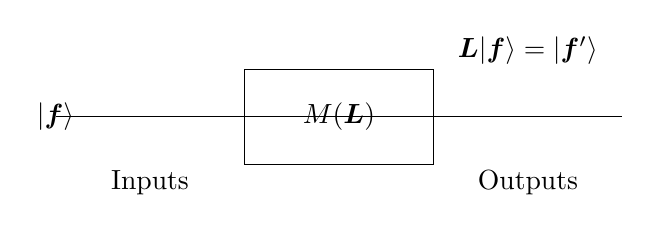
\begin{tikzpicture}[scale=1.2]
  % Baseline line
  \draw (0,0.5) -- (6,0.5);
  
  % Box
  \draw (2,0) rectangle (4,1);
  \node at (3,0.5) {$M(\bm{L})$};
  
  % Left label
  \node at (0,0.5) {$|\bm{f}\rangle$};
  \node at (1,-0.2) {Inputs};
  
  % Right label
  \node at (5,1.2) {$\bm{L}|\bm{f}\rangle = |\bm{f}'\rangle$};
  \node at (5,-0.2) {Outputs};
\end{tikzpicture}
\end{center}

\end{document}